%%%%%%%%%%%%%%%%%%%%%%%%%%%%%%%%%%%%%%%%%%%%%%%%%%%%%%%%%%%%%%%%%%%%%%%%%%%%%%%%%%%%%%%%%%%%%%%%%%%%%%%%%%%%%%%%%%%%%%%%%%%%%%%%%%%%%%%%%%%%%%%%%%%%%%%%%%%
% This is just an example/guide for you to refer to when submitting manuscripts to Frontiers, it is not mandatory to use Frontiers .cls files nor frontiers.tex  %
% This will only generate the Manuscript, the final article will be typeset by Frontiers after acceptance.
%                                              %
%                                                                                                                                                         %
% When submitting your files, remember to upload this *tex file, the pdf generated with it, the *bib file (if bibliography is not within the *tex) and all the figures.
%%%%%%%%%%%%%%%%%%%%%%%%%%%%%%%%%%%%%%%%%%%%%%%%%%%%%%%%%%%%%%%%%%%%%%%%%%%%%%%%%%%%%%%%%%%%%%%%%%%%%%%%%%%%%%%%%%%%%%%%%%%%%%%%%%%%%%%%%%%%%%%%%%%%%%%%%%%

%%% Version 3.4 Generated 2022/06/14 %%%
%%% You will need to have the following packages installed: datetime, fmtcount, etoolbox, fcprefix, which are normally inlcuded in WinEdt. %%%
%%% In http://www.ctan.org/ you can find the packages and how to install them, if necessary. %%%
%%%  NB logo1.jpg is required in the path in order to correctly compile front page header %%%

\documentclass[utf8]{FrontiersinHarvard} % for articles in journals using the Harvard Referencing Style (Author-Date), for Frontiers Reference Styles by Journal: https://zendesk.frontiersin.org/hc/en-us/articles/360017860337-Frontiers-Reference-Styles-by-Journal

\usepackage{url,hyperref,lineno,microtype,subcaption}
\usepackage[onehalfspacing]{setspace}

\linenumbers

% Leave a blank line between paragraphs instead of using \\

\def\keyFont{\fontsize{8}{11}\helveticabold }
\def\firstAuthorLast{Lee, Hadfield {et~al.}} %use et al only if is more than 1 author
\def\Authors{Jover Lee\,$^{1,\dagger}$, James Hadfield\,$^{1,\dagger}$, Allison Black\,$^{2}$, Thomas R. Sibley\,$^{1}$, Richard A. Neher\,$^{3,4}$, Trevor Bedford\,$^{1,5}$, and John Huddleston\,$^{1,*}$}
% Affiliations should be keyed to the author's name with superscript numbers and be listed as follows: Laboratory, Institute, Department, Organization, City, State abbreviation (USA, Canada, Australia), and Country (without detailed address information such as city zip codes or street names).
% If one of the authors has a change of address, list the new address below the correspondence details using a superscript symbol and use the same symbol to indicate the author in the author list.
\def\Address{$^{1}$Vaccine and Infectious Disease Division, Fred Hutchinson Cancer Center, Seattle, WA, USA \\
  $^{2}$Chan Zuckerberg Initiative, CA, San Francisco, CA, USA \\
  $^{3}$Biozentrum, Universität Basel, Switzerland \\
  $^{4}$Swiss Institute of Bioinformatics, Switzerland \\
  $^{5}$Howard Hughes Medical Institute, Seattle, WA, USA \\
  $^{\dagger}$These authors contributed equally to this work and share first authorship}
% The Corresponding Author should be marked with an asterisk
% Provide the exact contact address (this time including street name and city zip code) and email of the corresponding author
\def\corrAuthor{John Huddleston}
\def\corrEmail{jhuddles@fredhutch.org}

\begin{document}
\onecolumn
\firstpage{1}

\title[Joint visualization of influenza serology and phylogeny]{Joint visualization of seasonal influenza serology and phylogeny to inform vaccine composition}

\author[\firstAuthorLast ]{\Authors} %This field will be automatically populated
\address{} %This field will be automatically populated
\correspondance{} %This field will be automatically populated

\extraAuth{}% If there are more than 1 corresponding author, comment this line and uncomment the next one.
%\extraAuth{corresponding Author2 \\ Laboratory X2, Institute X2, Department X2, Organization X2, Street X2, City X2 , State XX2 (only USA, Canada and Australia), Zip Code2, X2 Country X2, email2@uni2.edu}

\maketitle

\begin{abstract}

\section{}

Seasonal influenza vaccines must be updated regularly to account for mutations that allow influenza viruses to escape our existing immunity.
A successful vaccine should represent the genetic diversity of recently circulating viruses and induce antibodies that effectively prevent infection by those recent viruses.
Thus, linking the genetic composition of circulating viruses and the serological experimental results measuring antibody efficacy is crucial to the vaccine design decision.
Historically, genetic and serological data have been presented separately in the form of static visualizations of phylogenetic trees and tabular serological results to identify vaccine candidates.
To simplify this decision-making process, we have created an interactive tool for visualizing serological data that has been integrated into Nextstrain's real-time phylogenetic visualization framework, Auspice.
We show how the combined interactive visualizations may be used by decision makers to explore the relationships between complex data sets for both prospective vaccine virus selection and retrospectively exploring the performance of vaccine viruses.

\tiny
 \keyFont{ \section{Keywords:} influenza, serology, phylogeny, interactive, visualization} %All article types: you may provide up to 8 keywords; at least 5 are mandatory.
\end{abstract}

\section{Introduction}

Seasonal influenza A/H3N2 viruses primarily evolve by acquiring mutations that allow them to escape antibodies from previous infections or vaccinations \citep{Petrova2018}.
This process, known as antigenic drift, changes the appearance of viral surface proteins hemagglutinin and neuraminidase.
Hemagglutinin (HA) is the primary target of our adaptive immunity and the primary component of the seasonal influenza vaccine.
Therefore, continued antigenic drift in HA necessitates regular updates to the seasonal influenza vaccine.

The World Health Organization (WHO) Global Influenza Surveillance and Response System (GISRS) tracks antigenic drift throughout the year by sequencing the HA gene of circulating viruses, growing candidate vaccine viruses in cell lines and chicken eggs, and performing serological experiments \citep{Morris:2017ea}.
HA gene sequences reveal ``clades'' or groups of recent influenza viruses that descend from a common ancestor.
When the common ancestor of a clade carries amino acid mutations in HA that have been previously associated with antigenic drift \citep{Wolf:2006da,Shih:2007bd,Koel:2013jz}, viruses in that clade may be able to escape our existing immunity.
GISRS researchers select representative viruses from major clades to grow in the cell line and chicken egg environments used in vaccine production \citep{Katz2011}.
Viruses that grow in these conditions become candidate vaccine viruses or vaccine candidates.
Serological experiments measure antigenic drift by quantifying how well viruses from one clade can escape detection by antibodies against vaccine candidates from the same clade or other clades.
These experimental measurements validate the effects of specific mutations on antigenic drift.

The gold standard of these serological experiments is the hemagglutination inhibition (HI) assay \citep{hirst1943studies}.
HI assays measure the minimum concentration or ``titer'' of antibodies required to prevent a given test virus from binding to red blood cells.
Typically, antibodies come from previously uninfected ferrets who are then infected with a specific reference virus (e.g., a vaccine candidate).
Each HI assay requires a series of two-fold dilutions of ferret antibodies to determine the minimum titer that inhibits binding.
The higher the antibody titer required to prevent binding, the more antigenically drifted the test virus is from the reference virus.
To enable comparison between measurements from different reference viruses, researchers normalize titers by the titer required to inhibit the reference virus itself and convert values to a $\log_{2}$ scale \citep{Neher:2016hy}.
The resulting values represent the magnitude of antigenic distance between a given reference virus and other test viruses.
Traditionally, viruses with an antigenic distance greater than $2\log_{2}$ units are considered antigenically distinct \citep{Katz2011}.

The WHO convenes influenza vaccine composition meetings (VCMs) twice per year with each meeting occurring approximately 9 months prior to the next influenza season in a given hemisphere \citep{Morris:2017ea}.
At these meetings, WHO decision makers must select a single vaccine virus for H3N2 from the pool of available vaccine candidates.
This selection strongly depends on the patterns of antigenic drift present in HI titers for clades identified from HA gene sequences.
Key questions that decision makers must answer in this process include a) which available vaccine candidates require additional titer measurements against currently circulating clades, b) which vaccine candidates have the lowest antigenic distance to each clade, and c) what is the antigenic diversity of recent clades?
The best vaccine candidate will have titer measurements against all current clades and have the lowest antigenic distance across these clades.
Such candidates are said to effectively ``cover'' currently circulating clades.
Determining the vaccine candidate that most effectively covers recent clades requires a direct comparison of antigenic distances across all available vaccine candidates.

Historically, WHO decision makers have answered the key questions above using standard phylogenetic visualizations \citep{felsenstein:2003,lemey:2012} and separate visualizations of antigenic evolution \citep{Smith:2004jc}.
Visualization of antigenic evolution in a phylogenetic context is a relatively recent development \citep{Steinbruck:2012ja,Bedford:2014bf,Neher:2016hy}.
We previously developed two alternate visualizations of antigenic data to inform vaccine selection through reports to the WHO \citep{BedfordWHO2018,BedfordWHO2019}.
The first visualization is an interactive phylogenetic view implemented in the genomic epidemiology tool \emph{nextflu} \citep{NeherBedford2015,NeherBedford2018}.
When the user selects a given reference virus from the phylogeny (by selecting a ``gear'' icon), the tool plots the pairwise antigenic distances between that reference and the corresponding test viruses in the tree using color to represent the distance values (Figure~\ref{fig:1}A).
This representation reveals clades that the selected reference virus may or may not cover and which clades lack measurements against the reference.
While this view provides phylogenetic context of titer measurements and shows the individual pairwise measurements, it does not support direct comparison of antigenic distances from different vaccine candidates.
Instead, users must quickly toggle between different vaccine candidates in the tree to get a sense of how well different viruses may perform.

To complement the interactive phylogenetic visualization, we also developed a static heatmap visualization that summarizes the mean antigenic distances between a subset of vaccine candidates and all test viruses within each extant clade.
The resulting heatmaps use the x-axis to encode the names of major clades, the y-axis to encode the names of reference viruses, and color and text to encode the mean $\log_{2}$ distance between a given reference virus and corresponding test viruses in each clade (Figure~\ref{fig:1}B).
These heatmaps allow decision makers to directly compare average antigenic distances for different vaccine candidates and quantify how well these candidates cover extant clades.
However, these heatmaps suffer reduced expressiveness by encoding the most valuable quantitative data with color instead of a positional encoding.
Additionally, this view shows a summary statistic instead of the underlying distributions of the data, concealing the number and variance of measurements for each reference virus.

To overcome the limitations of existing antigenic visualizations, we applied user-driven design based on the goals of decision makers described above and used standard visual design principles to produce a more expressive and effective visualization for influenza virologists.
The result is a new component of Nextstrain's interactive phylogenetic visualization platform that we call the measurements panel.
Below, we describe the measurements panel and provide two case studies that demonstrate the practical value of this tool for vaccine composition decisions.

\section{Methods}

\subsection{Visual design}

Of the two previous visualizations we developed, the static heatmaps addressed the most user goals except for communicating which extant clades were missing measurements.
Our two previous visualizations either obscured or hid the underlying distributions of the raw data.
Since visualization of these distributions can improve confidence during the decision-making process \citep{correll2014error,Hullman2015,Fernandes2018}, we treated the need to view these distributions as an auxiliary user goal.

In the context of visual design principles, both the phylogenetic and heatmap views encode the most relevant quantitative data of antigenic distance with color.
However, quantitative data can be more effectively represented by positional encodings (e.g., x- or y-axis positions) whereas nominal data (e.g., names of phylogenetic clades) can be effectively encoded with color \citep{Mackinlay1986}.
In \emph{nextflu}'s phylogenetic view, the two available positional axes represent time and the unitless phylogenetic position of nodes, neither of which are relevant to the user goals described above.
In the heatmaps, the two positional axes encode two nominal data types.

We reasoned that we could make a more effective visualization that addressed all user goals by simply changing the encoding of data in the heatmaps.
To this end, we swapped the encoding of antigenic distances and test clades, encoding quantitative distances on the x-axis positional scale and encoding nominal test clades with a color scale.
The positional encoding of antigenic distances allowed us to visually encode relevant thresholds for decision-making (e.g., $x = 2\log_{2}$), show all available measurements for each reference virus at once, and display a summary statistic (mean and standard deviation of antigenic distances) for each reference virus.
We retained the encoding of nominal reference virus names on the y-axis, since most user goals require comparison of distances between specific vaccine candidates.

\subsection{Implementation}

We implemented this design as a new interactive measurements panel within Nextstrain's visualization tool, Auspice, which is freely available on GitHub (\href{https://github.com/nextstrain/auspice}{github.com/nextstrain/auspice}) under the AGPLv3 license.
Auspice is a phylogenetic visualization platform inspired by \emph{nextflu} and which maintains the interactive data exploration, with the measurement panel appearing alongside and in-sync with other views into the data (currently phylogenetic, geographic and genomic diversity views).
The visualization requires a minimum of two JavaScript Object Notation (JSON) files that are produced by the Nextstrain bioinformatics toolkit, Augur \citep{Huddleston2021}.
The phylogenetic tree is provided via a dataset JSON file produced by \texttt{augur export v2} and the measurements data is provided via a measurements sidecar JSON file produced by \texttt{augur measurements}.
The measurements file must follow a specific filename format for Auspice to link it to the dataset file, where the dataset filename is \texttt{\$\{name\}.json} and the measurements filename must be \texttt{\$\{name\}\_measurements.json}.
The application can be cloned and run locally or users can use Auspice through two public websites.
Users can drag and drop dataset and measurements files onto \href{https://auspice.us/}{auspice.us/} to visualize the data locally in their own browser.
Visualizations can be also shared with others through \href{https://nextstrain.org/}{nextstrain.org/} (the data presented in this paper is available at \href{https://nextstrain.org/community/blab/measurements-panel/flu/seasonal/h3n2/ha}{nextstrain.org/community/blab/measurements-panel/flu/seasonal/h3n2/ha}).
Full documentation for sharing analyses through Nextstrain can be found at \href{https://docs.nextstrain.org/page/guides/share/}{docs.nextstrain.org/page/guides/share/}.

\subsection{Data curation and analysis}

We evaluated the new measurements panel by constructing a Nextstrain analysis \citep{Hadfield2018} with previously published HA gene sequences and HI titers \citep{Bedford:2014bf}.
A full data curation guide is available online at \href{https://github.com/blab/measurements-panel/tree/main/data#readme}{github.com/blab/measurements-panel/tree/main/data\#readme} and a full guide to running the bioinformatics analyses is available at \href{https://github.com/blab/measurements-panel#readme}{github.com/blab/measurements-panel\#readme}.
Briefly, we downloaded HI titer data and accessions for H3N2 HA sequences from \cite{Bedford:2014bf}'s GitHub repository.
We downloaded and combined HA sequences from the Influenza Virus Resource or GISAID, depending on the original source.
We parsed metadata including viral sample name, database accession, collection date, and sequence authors from the sequence headers with \texttt{augur parse}.
We aligned HA sequences with mafft v7.508 \citep{Katoh2013}, inferred a phylogenetic tree with IQ-TREE 2.2.0.3 \citep{Minh2020}, and inferred a time tree with TreeTime 0.9.4 \citep{Sagulenko2018}.
We annotated mutations on the phylogenetic tree and constructed the measurement panel data JSON with Augur 18.0.0 \citep{Huddleston2021}.
For improved reproducibility, we automated the execution of these tasks in a Snakemake workflow \citep{Molder2021}.
In the absence of official WHO clade designations for the time period of this analysis, we manually defined clades based on amino acid mutations at HA positions previously associated with antigenic drift \citep{Wolf:2006da} that also led to later successful lineages in the HA phylogenetic tree.
We also selected these clades to represent enough genetic diversity of HA through time to highlight the measurement panel's functionality of grouping data by clade.
To construct the measurements panel JSON, we normalized the raw HI titer measurements with Augur's implementation of the titer substitution model \citep{Neher:2016hy}, converted these measurements to a tab-separated values (TSV) file with a custom Python script, and ran the new \texttt{augur measurements export} command with this TSV file as input.
The resulting visualization for this paper has been shared via Nextstrain community and can be viewed at \href{https://nextstrain.org/community/blab/measurements-panel/flu/seasonal/h3n2/ha}{nextstrain.org/community/blab/measurements-panel/flu/seasonal/h3n2/ha}.

\section{Results}

\subsection{Interactive visualization of titer measurements}

Our goal for incorporating the measurements panel into Auspice is to allow users to explore relationships between the genetic and serological data in one interactive visualization.
Test viruses of the titer data are directly linked by name to the viruses displayed in the phylogenetic tree, to ensure that any interactions with the tree also affect the measurements displayed.
When users filter the tree by date (Figure~\ref{fig:2}a), metadata attributes of viruses (Figure~\ref{fig:2}d), or subtrees selected by clicking on a corresponding tree branch, the measurements panel updates to reflect only the matching test viruses.
Users can easily focus on a subset of phylogenetically relevant measurements and examine the measurements of test viruses in recently circulating clades.
The measurements are colored by the same coloring attribute (Figure~\ref{fig:2}b) as the phylogenetic tree, adding the legend values (Figure~\ref{fig:2}c) as another dimension of nominal data to the titer measurements.
This coloring is especially useful for viewing titer data by genotypes of test viruses, allowing users to inspect relationships between specific mutations in HA and antigenic drift quantified by titer measurements.
The investigation of genotypes is further facilitated by the diversity panel in Auspice, which shows the diversity of alleles across the genome.
Clicking on a bar in the diversity panel will change the coloring of the tree and measurements to the genotypes at that position (Figure~\ref{fig:2}n).

The measurements JSON can include multiple collections of titers for a single phylogenetic tree and users can change the collection displayed with the collection dropdown (Figure~\ref{fig:2}e).
Users can then review different sets of data for the same phylogenetic tree such as separate measurements of cell- and egg-passaged virus titers.
Within each collection, users can compare measurements across different groupings by changing the grouping category with the ``group by'' dropdown (Figure~\ref{fig:2}f).
For vaccine selection, grouping by the reference virus (Figure~\ref{fig:2}j) allows decision makers to directly compare titers across multiple vaccine candidates.
Other groupings such as data source or ferret serum can be used to explore the variability of the titer measurements.
The overall mean for each grouping can then be toggled (Figure~\ref{fig:2}h) for whole group comparisons.

The data display can be switched between mean with standard deviation and raw individual measurements (Figure~\ref{fig:2}g).
The means are calculated per color attribute to allow for comparisons across attributes within each group.
This view maintains the ability to view the mean antigenic distance for test viruses within each clade that we had implemented in the static heatmaps.
The raw measurements view plots each individual measurement to give users a detailed view of the quantity and distribution of titers, which can inform design decisions for future titer experiments.
The titers threshold can be toggled (Figure~\ref{fig:2}i) to add a clear demarcation of the threshold value for a binary view of when titer measurements are considered antigenically distinct (Figure~\ref{fig:2}k).
We discuss the application of these features in detail in two case studies in the following sections.

\subsection{Case study 1: Retrospective vaccine selection in fall 2009}

As noted above, the WHO convenes VCMs twice per year \citep{Morris:2017ea}.
The northern hemisphere VCM occurs in February or March ahead of a winter season in October through April.
The southern hemisphere VCM occurs in September or October ahead of a winter season in April through October.
To demonstrate the utility of an interactive visualization of serological measurements for vaccine composition decisions, we performed a retrospective analysis of a H3N2 vaccine update made for the southern hemisphere in the fall of 2009.
We used publicly available sequence and titer data \citep{Bedford:2014bf} to reconstruct a H3N2 HA phylogeny and measurements panel representing information that was available at the time of the VCM (see Methods).
We note that the actual selection process used a richer dataset which is not publicly available to include here, and as such these data should be seen as representative of the process only.

The VCM ahead of the 2010 southern hemisphere season occurred in September 2009.
Three clades circulated at that time including 173Q and two of its subclades named 144K and 158N/189K (Figure~\ref{fig:3}A).
The most recent H3N2 vaccine virus, A/Brisbane/10/2007, had been used for the two prior influenza seasons (2008 and 2009) and represented an older clade, 140I, that had since been replaced by 173Q \citep{WHO:archive}.
Prior to the A/Brisbane/10/2007 vaccine, A/Wisconsin/67/2005 had been the vaccine virus in the 2007 southern hemisphere season.
While 173Q dominated the 2008-2009 season, 144K appeared to be dominant in September 2009.
At the time of the VCM, titers for both A/Brisbane/10/2007 and A/Wisconsin/67/2005 against test viruses from 144K and 158N/189K exceeded the $2\log_{2}$ threshold (Figure~\ref{fig:3}B), indicating their inability to cover these recent clades.
In contrast, a newer vaccine candidate from the 144K clade, A/Perth/16/2009, had mean titers less than $1\log_{2}$ against the same recent clades.
These results strongly supported an update from the previous vaccine virus to a vaccine based on A/Perth/16/2009.
The WHO announced this decision on September 25, 2009.

Our retrospective analysis allows us to see how the evolution of H3N2 continued after the VCM decision.
Data collected after the vaccine selection deadline show that clade 158N/189K dominated for the following H3N2 seasons in both hemispheres (Figure~\ref{fig:3}A).
Although later HI measurements show that A/Perth/16/2009 did not cover viruses from 158N/189K as effectively as viruses from its own 144K clade (with mean $log_{2}$ values exceeding 1), the new vaccine was still a better antigenic match than the previous two vaccines (Figure~\ref{fig:3}C).
A/Perth/16/2009 remained the WHO's recommended H3N2 vaccine virus for the 2010-12 southern hemisphere seasons and the 2010-11 and 2011-12 northern hemisphere seasons \citep{WHO:recent}.

\subsection{Case study 2: Identification of genotype-specific patterns through visualization of raw data}

Influenza researchers often define clades of H3N2 viruses based on the presence of mutations that have been previously shown to enable viruses to escape existing immunity \citep{Wolf:2006da,Shih:2007bd,Koel:2013jz}.
The genetic similarity of viruses in the same clade typically corresponds with antigenic similarity of the same viruses as measured by HI assays.
However, new mutations may arise within a clade that cause test viruses with those mutations to differ antigenically from earlier viruses in the same clade.
Here, we demonstrate how aggregation of antigenic distances by clade can obscure the emergence of antigenically novel test viruses and how visualization of raw measurements can reveal these important patterns.

Using the same data from the previous case study, we noted that clade 144V circulated between 1984 and 1992 (Figure~\ref{fig:4}A) and that multiple HI measurements existed for reference and test viruses from this clade.
We identified two reference viruses in 144V with similar average HI measurements and divergent raw distributions (Figure~\ref{fig:4}B).
A/Shanghai/11/1987 had a mean antigenic distance of 1.64 $\pm$ 2.53 units, while A/Beijing/353/1989 had a mean distance of 1.13 $\pm$ 1.42 units.
The distributions of raw HI measurements revealed a bimodal distribution for A/Shanghai/11/1987 data and a unimodal distribution for A/Beijing/353/1989 (Figure~\ref{fig:4}C).
We hypothesized that antigenic mutations could explain the two clusters of test viruses in the A/Shanghai/11/1987 data.

We observed that position HA1:135 had the highest diversity among the 144V HA gene sequences in the diversity panel, indicating more distinct amino acid mutations at this position.
This position was previously identified as a putative antigenic site in HA where mutations could enable escape from existing immunity \citep{Wolf:2006da}.
Based on this genetic information, we colored the HI measurements by the genotypes of the test viruses at this position.
The genotype-specific coloring showed three different alleles at position 135 including the ancestral 135G and two derived alleles of 135E and 135D (Figure~\ref{fig:4}D).
This view also revealed that test viruses with same 135G genotype as A/Shanghai/11/1987 had lower antigenic distances (mean of -1.00 $\pm$ 1.34 units), while viruses with the derived 135E and 135D genotypes had higher antigenic distances (3.74 $\pm$ 0.69 and 2.73 $\pm$ 0.89, respectively).
Measurements against A/Beijing/353/1989 showed the inverse pattern with lower distances from this reference to test viruses with 135E and 135D (0.46 $\pm$ 0.79 and 0.72 $\pm$ 0.71, respectively) and higher distances to 135G (3.05 $\pm$ 1.18).

These results demonstrate how summary statistics can obscure biologically relevant patterns in the raw data.
They also show how the ability to interactively color data by different viral attributes like genotype can produce hypotheses to explain the patterns we see in the raw data.
Importantly, these results do not confirm that the differences we observe in antigenic distances were caused by mutations at HA1:135.
The same test viruses with derived 135 mutations also have mutations at two positions adjacent to HA's receptor binding site, HA1:145 and 193, where mutations have been previously shown to cause antigenic drift \citep{Koel:2013jz}.
Confirmation of mutational effects requires further experimental work.
However, this interactive visualization tool enables decision makers to explore their data and generate new hypotheses in ways that previous tools did not.

\section{Discussion}

Updating the seasonal influenza vaccine composition is a complex process that requires the synthesis of genetic and serological data and the interpretation of these data by a panel of international experts.
Effective visualizations facilitate both the synthesis and interpretation by presenting data in a biologically meaningful context.
Our interactive visualization tool presents serological data with a phylogenetic context, enabling decision makers to directly compare the antigenic distances between vaccine candidates and investigate patterns in the raw data.
This tool regularly informs our discussions of influenza evolution with our collaborators in GISRS.
Please note that the data presented here is a small subset of those used to inform vaccine selection due to data sharing restrictions; we support public sharing of data (where appropriate) as this enhances the usability and reach of tools such as this.


The move beyond static presentations of analyses towards interactive applications such as this facilitates more widespread usage and analysis of biological data.
Specifically, the ability to link static views of the data, such as those found in VCM reports, with URLs that allow an interactive view into the data as presented in the figure is an important bridge between researchers.
We hope that the adoption and continued development of biologically-informed visualization tools like this will facilitate a better understanding of pathogen evolution.

The benefits of integrated and interactive visualization of genetic and experimental data extend beyond serological measurements for seasonal influenza.
High-throughput experimental measurements of mutational effects and immune escape in both seasonal influenza and SARS-CoV-2 have required custom tools for visualization and interpretation of these high-dimensional data \citep{Hilton2020,Aksamentov2021,Garrett2021,Greaney2022}.
The data visualization presented here is amenable to showing similar multi-dimensional data, for instance linking different models to their scores across leaves in the phylogenetic tree in much the same way we have linked reference viruses to their titer measurements.
The data structure for the measurements panel is purposefully agnostic to the pathogen or data generation approach.
As research continues on the emergence of human pathogens from natural reservoirs in other organisms \citep{Olival2017,Leendertz2016} and high-dimensional experimental measurements of these pathogens accumulate \citep{Soh2019,Starr2022}, this flexible data structure and the resulting interactive visualizations could impact decision-making related to pandemic preparedness.

\section*{Conflict of Interest Statement}
%All financial, commercial or other relationships that might be perceived by the academic community as representing a potential conflict of interest must be disclosed. If no such relationship exists, authors will be asked to confirm the following statement:

The authors declare that the research was conducted in the absence of any commercial or financial relationships that could be construed as a potential conflict of interest.

\section*{Author Contributions}

JL, TRS, TB, and JHa designed and implemented the measurements panel in Auspice.
JHu and AB designed and implemented initial prototypes of interactive measurements visualizations.
JHu, AB, and RAN designed and implemented static visualizations.
JL, JHu, and JHa wrote the manuscript.

\section*{Funding}

This work was supported by NIH 75N93021C00015.
TB is an Investigator of the Howard Hughes Medical Institute.

\section*{Acknowledgments}

This work started as a project for University of Washington (UW) class CSE 512 Data Visualization as a part of the UW eScience Advanced Data Science Option curriculum and we would like to thank Dr.\ Jeffrey Heer, Halden Lin, and Dr.\ Jane Hoffswell for their input on the initial design.
We thank the members of GISRS for the high quality sequence and serological data used in this work.
We have annotated sequence authors whenever that information was available at \href{https://github.com/blab/measurements-panel/blob/main/data/h3n2_ha_metadata.tsv}{github.com/blab/measurements-panel/blob/main/data/h3n2\_ha\_metadata.tsv}.
Without open data sharing, this work would not be possible.

\section*{Data Availability Statement}

Details about how to prepare and analyze the data in this study live on GitHub at \href{https://github.com/blab/measurements-panel/}{github.com/blab/measurements-panel} and the dataset therein may be visualized via \href{https://nextstrain.org/community/blab/measurements-panel/flu/seasonal/h3n2/ha}{nextstrain.org/community/blab/measurements-panel/flu/seasonal/h3n2/ha}.

\bibliographystyle{Frontiers-Harvard}
\bibliography{measurements-panel}

%%% Make sure to upload the bib file along with the tex file and PDF
%%% Please see the test.bib file for some examples of references

\section*{Figure captions}

%%% Please be aware that for original research articles we only permit a combined number of 15 figures and tables, one figure with multiple subfigures will count as only one figure.
%%% Use this if adding the figures directly in the mansucript, if so, please remember to also upload the files when submitting your article
%%% There is no need for adding the file termination, as long as you indicate where the file is saved. In the examples below the files (logo1.eps and logos.eps) are in the Frontiers LaTeX folder
%%% If using *.tif files convert them to .jpg or .png
%%%  NB logo1.eps is required in the path in order to correctly compile front page header %%%

\begin{figure}[h!]
  \begin{center}
    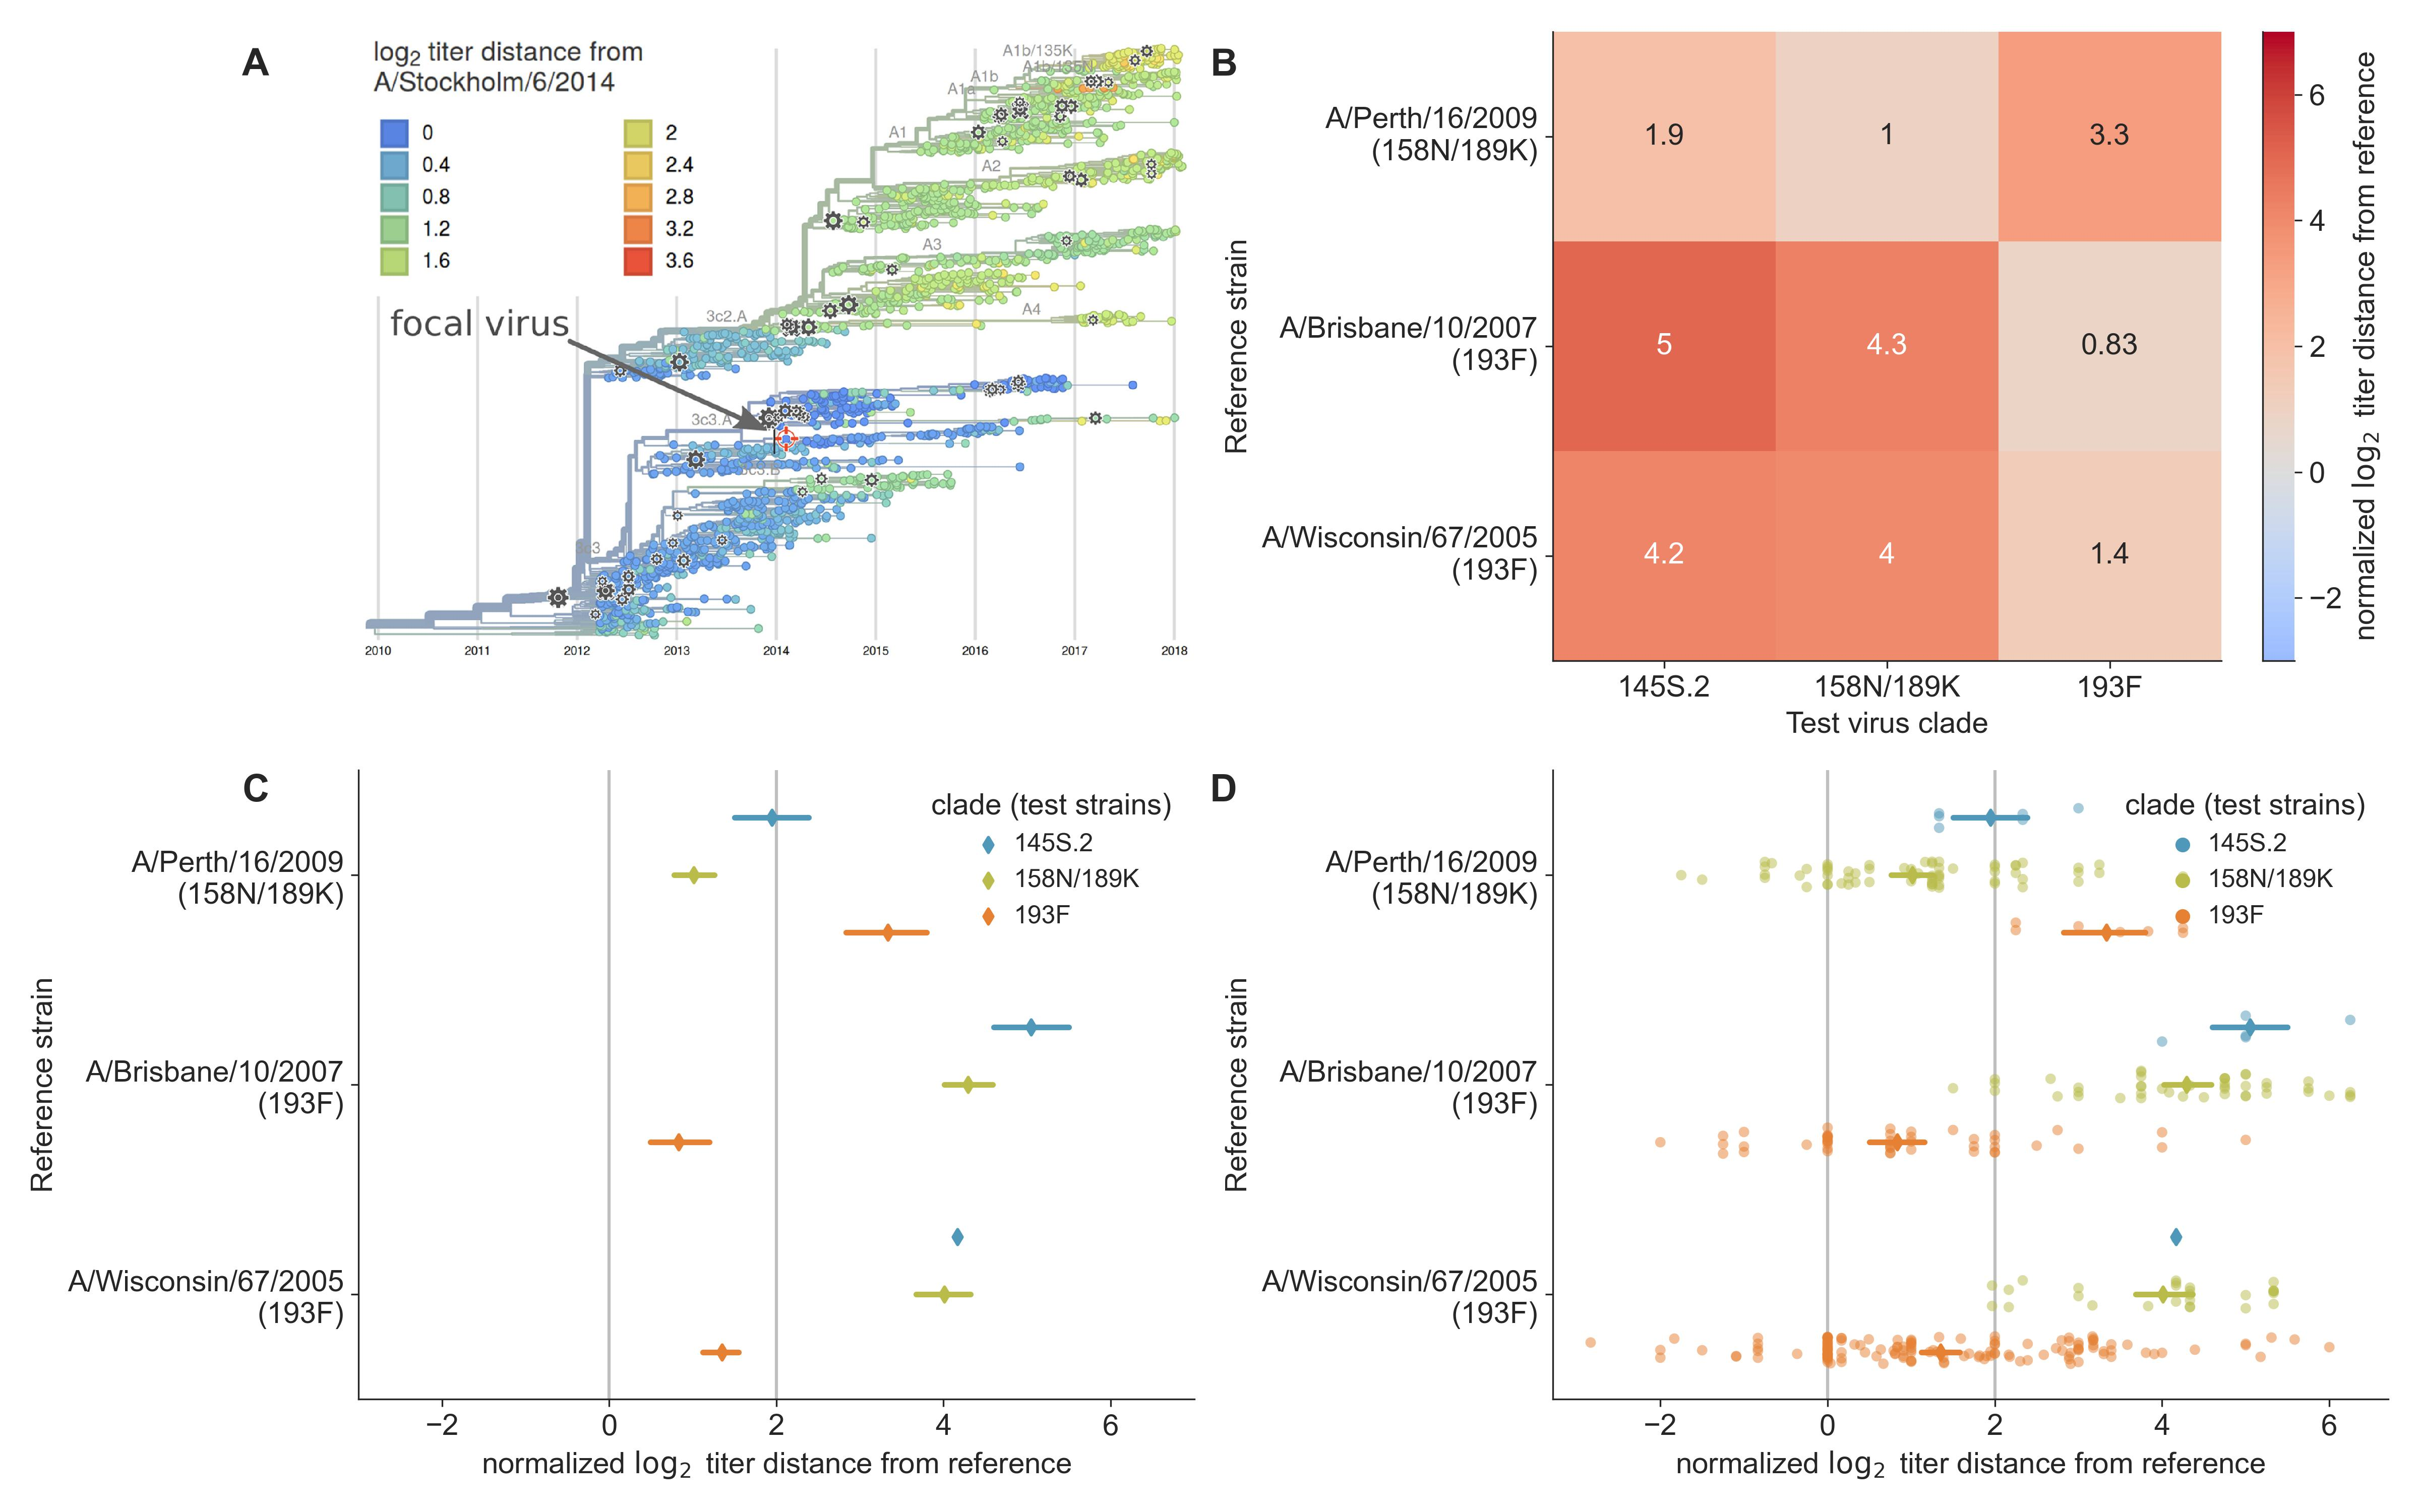
\includegraphics[width=\textwidth]{figures/figure-1-static-titer-visualizations}
  \end{center}
  \caption{
    Previous approaches to static visualization of serological data for seasonal influenza vaccine composition reports.
A) Phylogenetic visualization \citep{NeherBedford2018} allows the user to select a single vaccine candidate (e.g., A/Stockholm/6/2014) and see how well that virus might cover other circulating viruses in their genetic context based on the antigenic distance encoded by color (orange and red color indicate greater distance and less coverage by the selected virus).
To compare multiple vaccine candidates, users have to select different reference viruses manually and toggle between them.
B) Heatmap visualization of mean antigenic distances between multiple vaccine candidates (reference viruses on the y-axis) and viruses in currently circulating phylogenetic clades.
Heatmaps encode distance by color and text, allowing the user to compare how well multiple vaccine candidates might cover circulating viruses.
C) Interval plot of mean $\pm$ 89\% confidence interval values of antigenic distances between vaccine candidates (y-axis) and viruses in currently circulating clades.
Unlike the heatmap visualization, the interval plot encodes distance with a positional encoding (the x-axis) instead of color and encodes clades with color.
The vertical gray lines represent the threshold above which viruses are considered antigenically distinct (x=2, solid line) and where viruses are antigenically identical (x=0, dashed line).
This view allows users to compare multiple vaccine candidates, identify the candidate that covers specific clades based on a mean value to the left of the threshold at x=2, and view the variance in the underlying HI measurements.
D) Combined swarm and interval plot showing the raw pairwise measurements between each vaccine candidate and the test viruses in each clade.
This view allows users to perform the same tasks as the interval plot, but it also allows users to identify how many measurements support the summary statistics for a given vaccine candidate and identify multiple modes in the raw data distribution that could indicate within-clade antigenic variation.
}\label{fig:1}
\end{figure}

\begin{figure}[h!]
  \begin{center}
    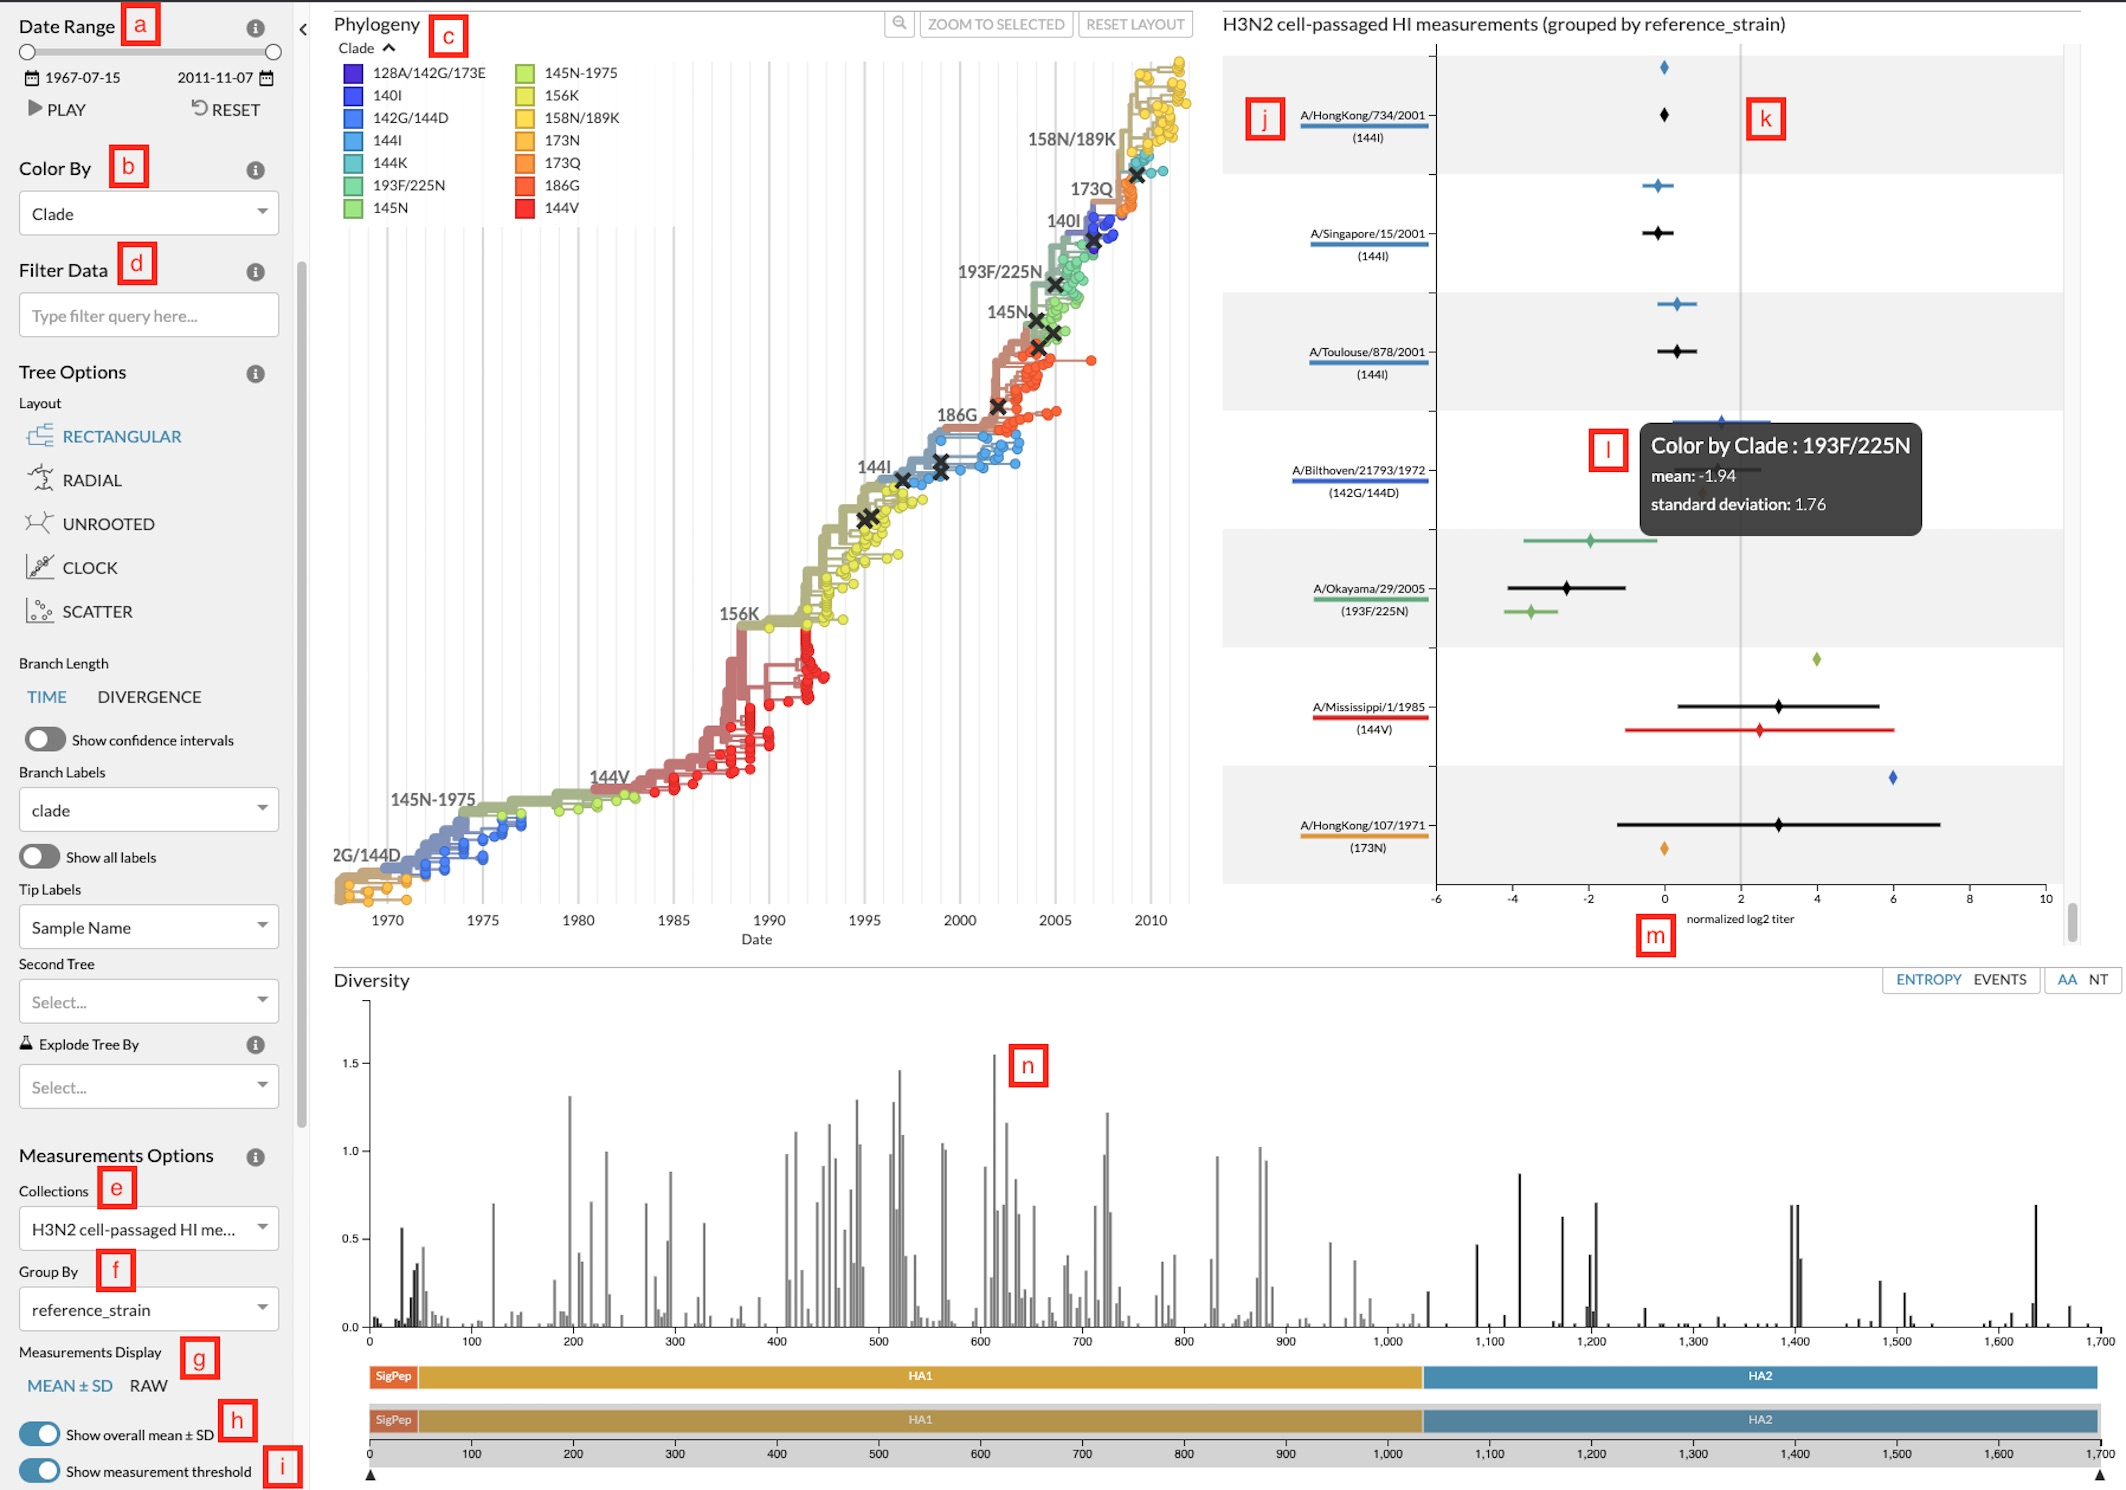
\includegraphics[width=\textwidth]{figures/figure-2-screen-shot}
  \end{center}
  \caption{
    Screenshot of Auspice with the sidebar controls, the phylogenetic tree panel, the measurements panel, and the diversity panel.
a) Date range slider to filter both tree and measurements by the test virus sample date.
b) Color-by dropdown to change the attribute to use for coloring the tree and measurements.
c) Legend for colors and their corresponding values linked to viruses in the tree and measurements.
d) Data filter search bar to filter tree and measurements data by specific attributes.
e) Measurements collection dropdown to change the collection of measurements displayed.
f) Measurements group by dropdown to change the grouping of measurements data.
g) Toggle to change measurements display between mean with standard deviation and individual raw measurements.
h) Toggle to display or hide the overall mean and standard deviation for each group.
i) Toggle to display or hide the threshold line.
j) Grouping label for each group of measurements.
This particular view uses reference viruses that are also present in the tree so the label includes the virus's corresponding color and color-by value.
k) The threshold line for titer measurements to indicate the threshold for antigenically distinct viruses.
l) The tooltip that displays more details for the hovered measurement.
This particular view hovers over a mean and standard deviation.
m) The x-axis of the measurements plot shows the range of measurements values in this collection.
n) Clicking on a bar in the diversity panel updates the tree and measurements to color by genotypes at that position.
  }\label{fig:2}
\end{figure}

\begin{figure}[h!]
  \begin{center}
    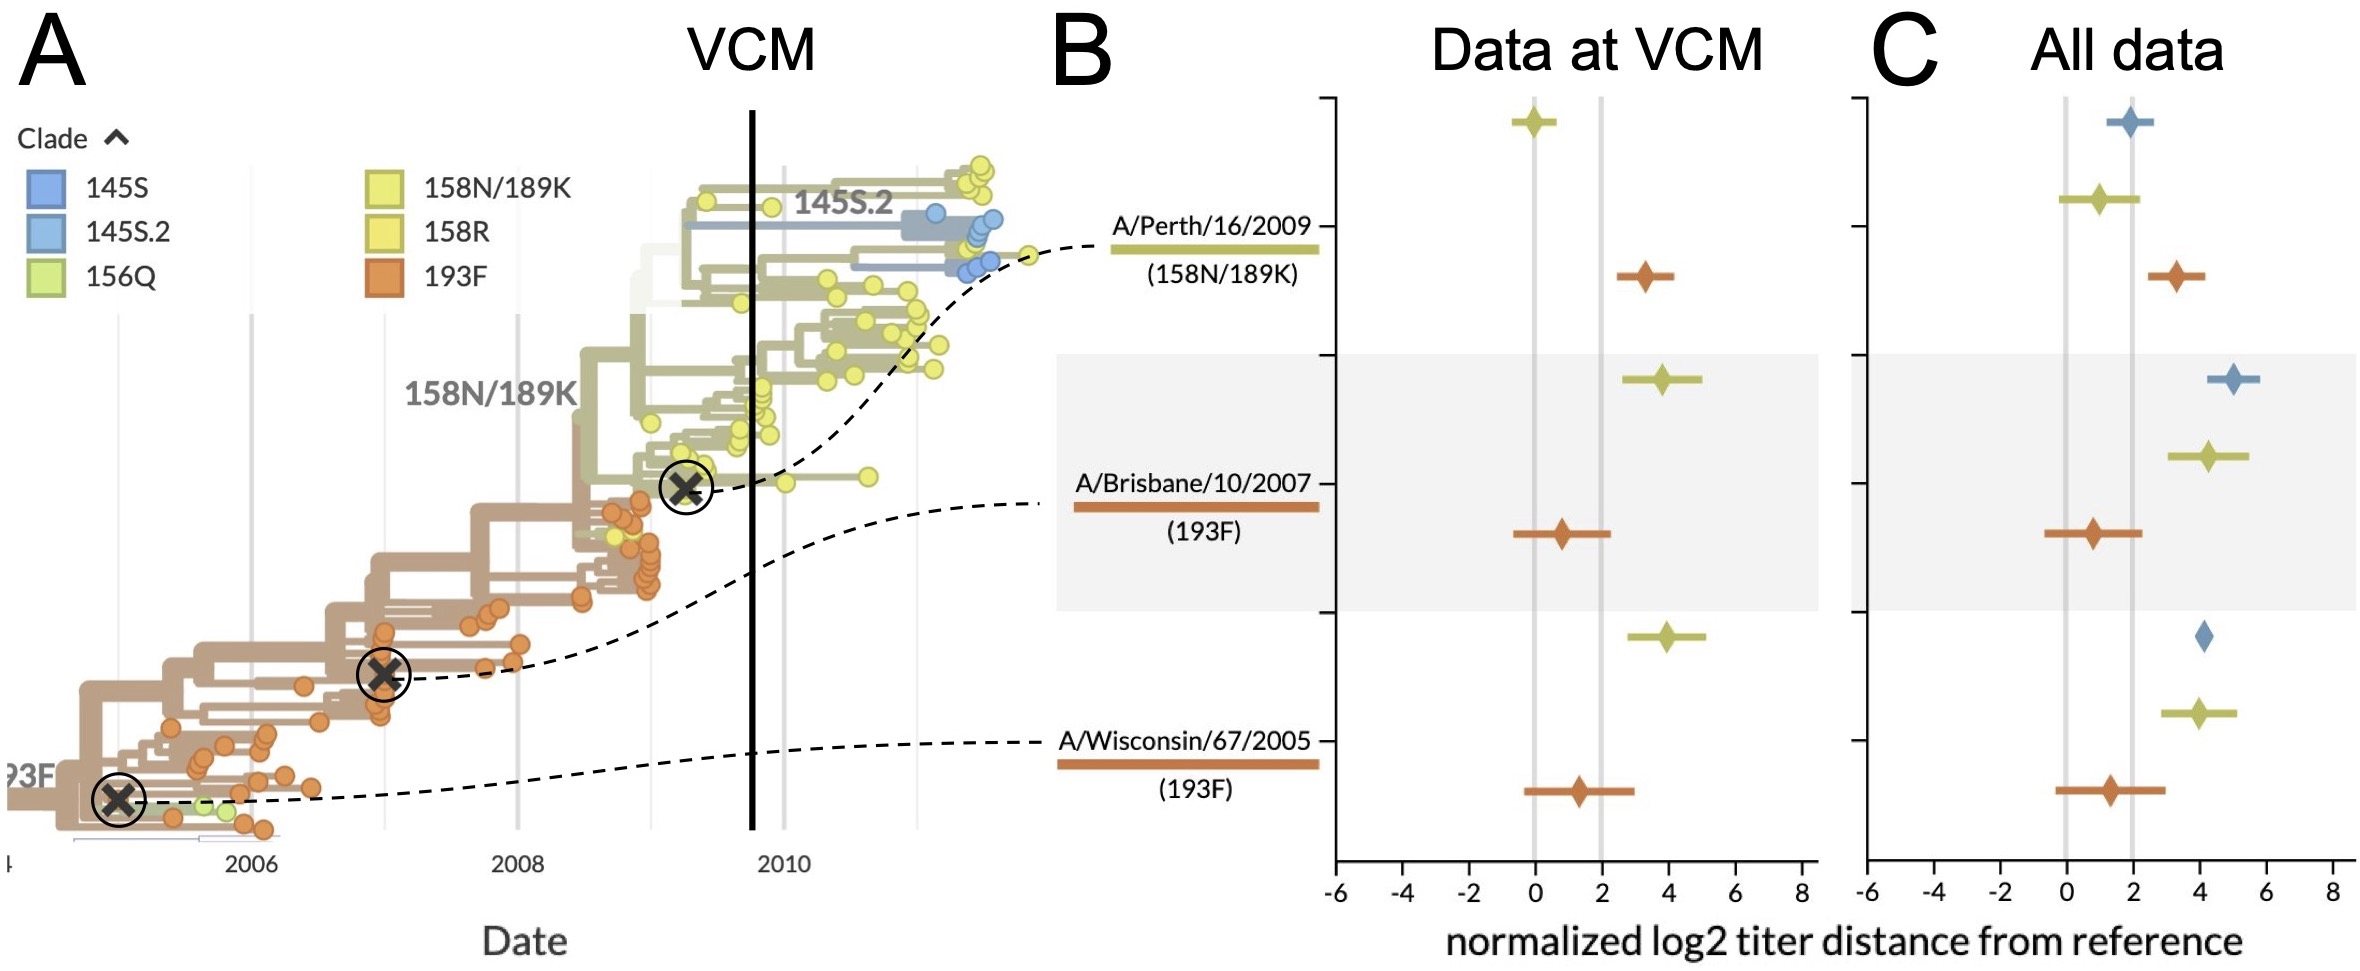
\includegraphics[width=\textwidth]{figures/figure-3}
  \end{center}
  \caption{
    Serological analysis of H3N2 clades around the time of the southern hemisphere vaccine composition meeting (VCM) for the 2010 influenza season.
    A) Phylogenetic tree summarizing the clades circulating before and after the VCM in September 2009.
    At the time of the VCM, clade 144K (light blue) was dominant, and A/Perth/16/2009 was the vaccine candidate from this clade.
    A/Brisbane/10/2007 (clade 140I) had been the southern hemisphere vaccine in 2008 and 2009 and A/Wisconsin/67/2005 (clade 193F/225N) had been the vaccine in 2007.
    B) HI titers against three vaccine candidates, using only data available prior to the final decision from the VCM (September 25, 2009).
    HI titers greater than $2\log_{2}$ indicate the inability of previous vaccines to cover viruses from the most recent clades.
    C) Same as (B) but including test viruses and HI measurements collected after the VCM, which were mainly from clade 158N/189K.
    With mean HI titers less than $2\log_{2}$, A/Perth/16/2009 covered this successful clade better than the previous vaccines.
  }
  \label{fig:3}
\end{figure}

\begin{figure}[h!]
  \begin{center}
    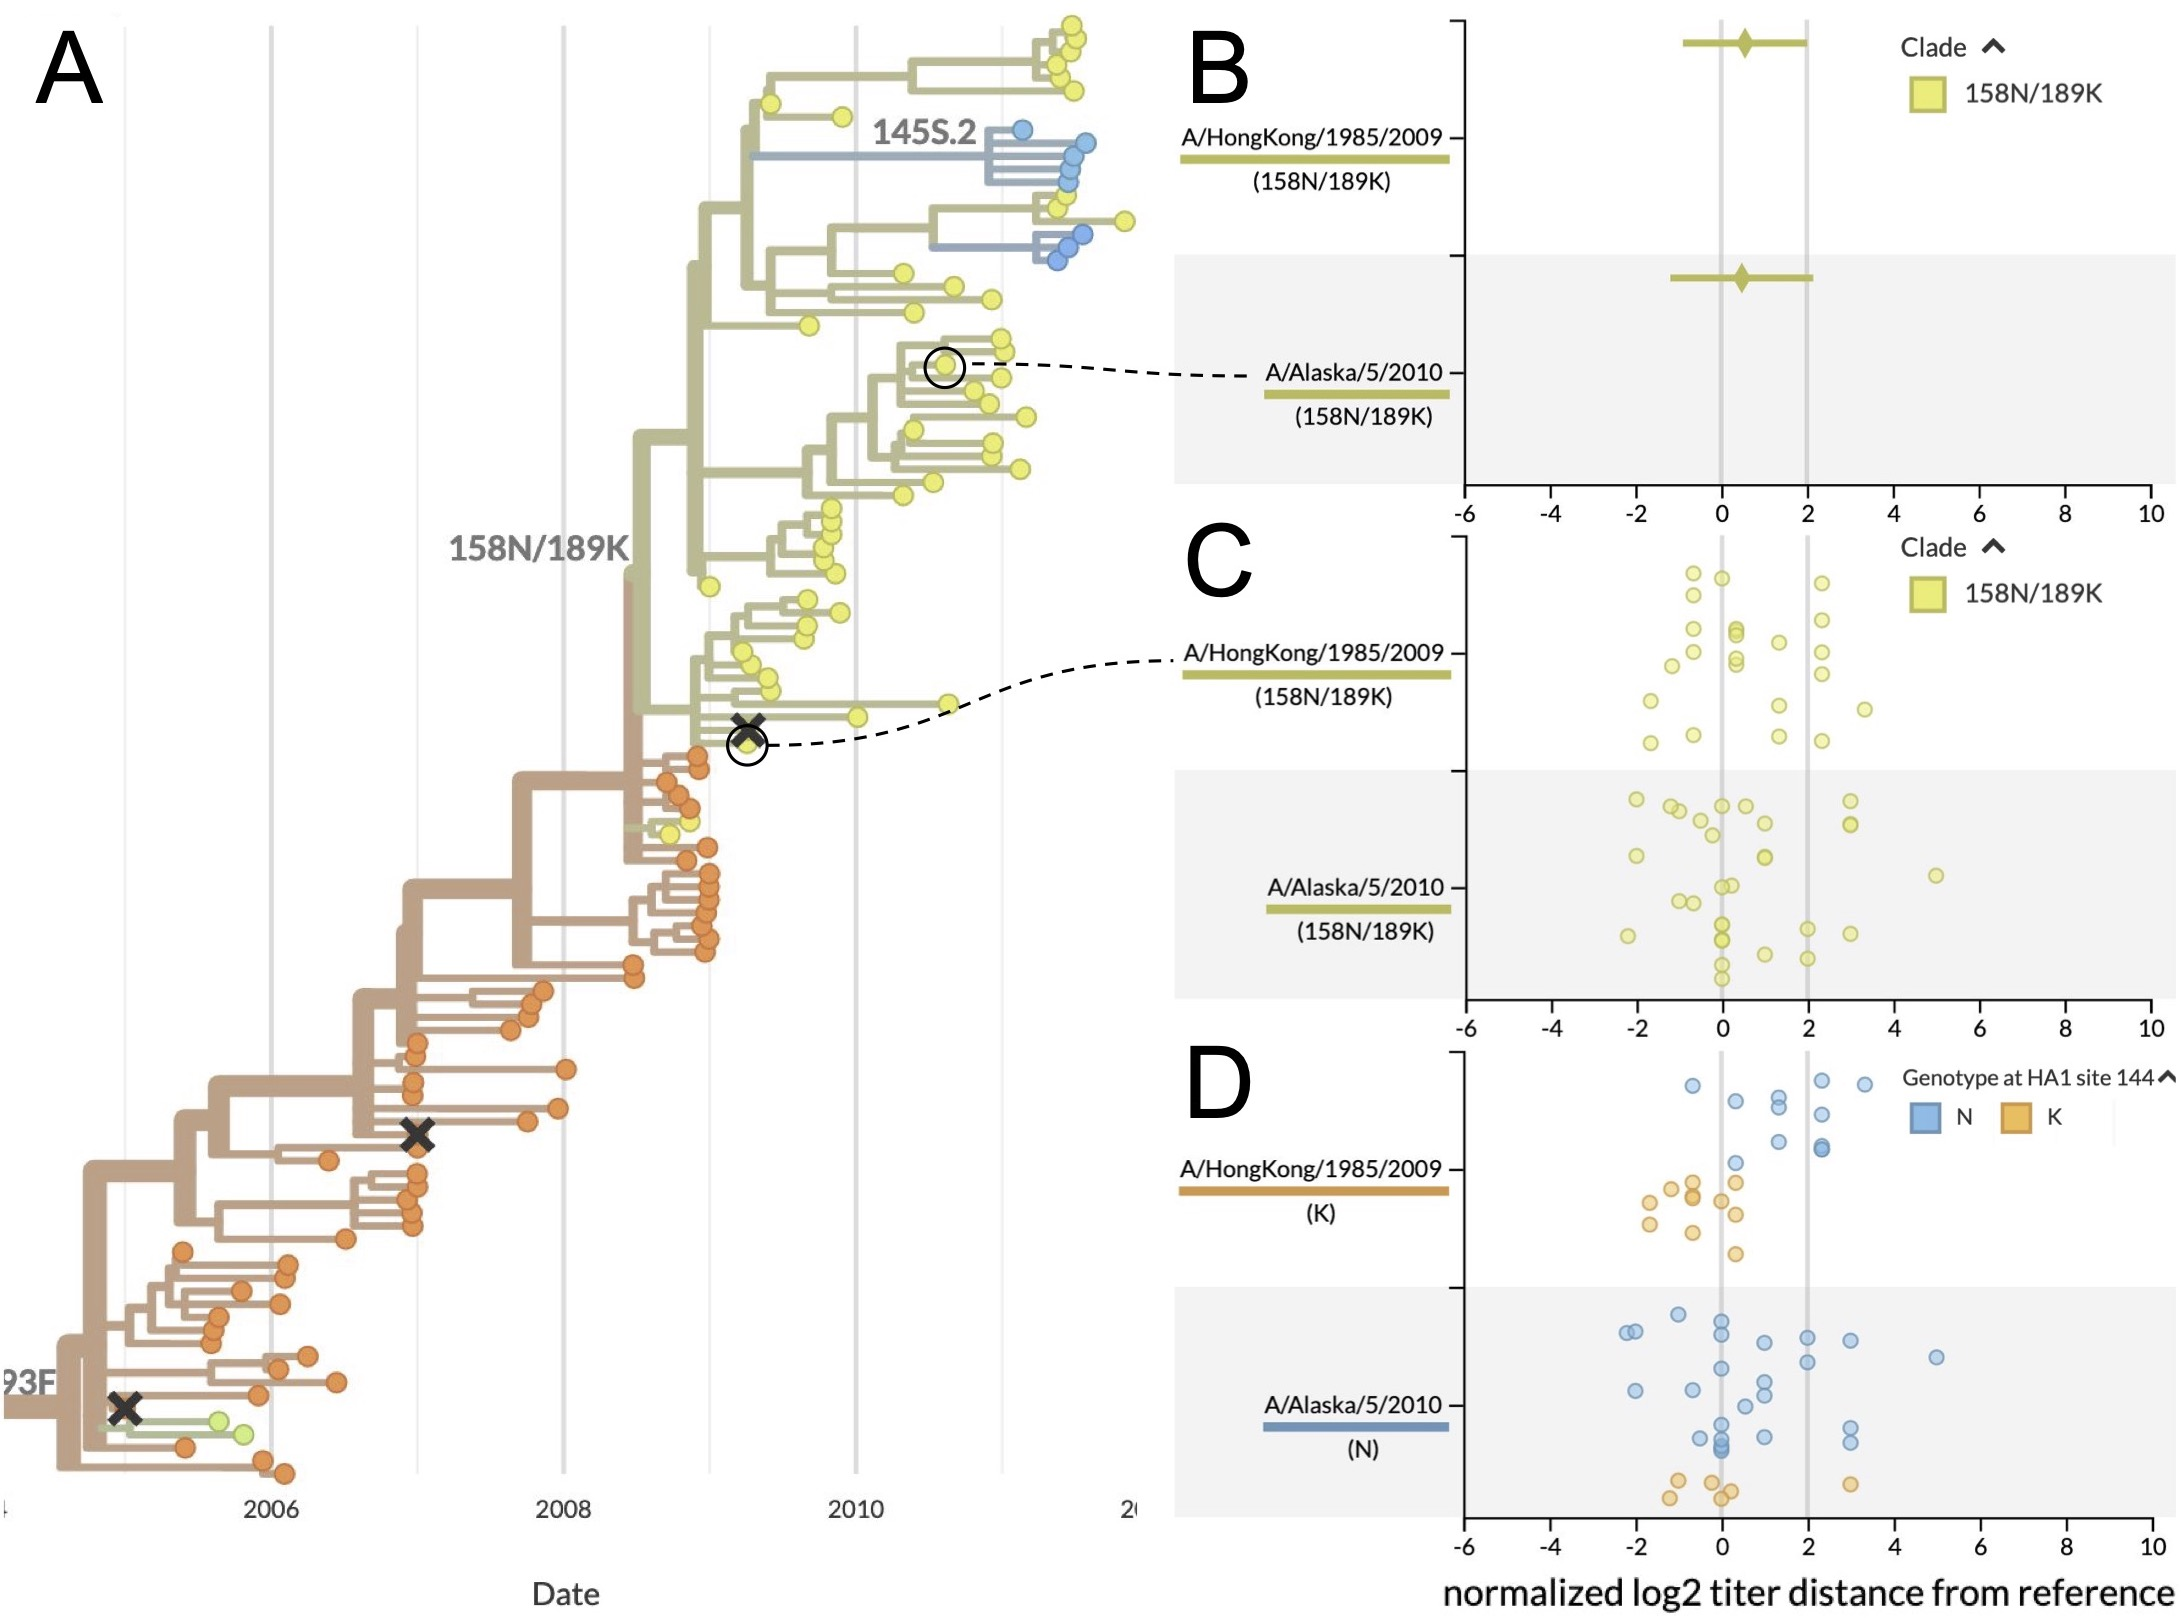
\includegraphics[width=\textwidth]{figures/figure-4}
  \end{center}
  \caption{
    Antigenic distances from HI assays between clade 144V reference and test viruses, highlighting two reference viruses with similar mean distances and divergent raw distributions.
    A) Summary phylogenetic tree with clade 144V highlighted in red.
    B) HI measurements when viewed as mean $\pm$ standard deviation show similar average values for two reference viruses and a wide range of antigenic diversity per reference.
    C) Viewing the individual measurements reveals a previously hidden bimodal distribution in the measurements for the A/Shanghai/11/1987 reference virus compared to an apparently unimodal distribution for the A/Beijing/353/1989 reference virus.
    D) Coloring individual measurements by genotypes at the putative antigenic site HA1:135 shows a potential genotype-specific explanation for the two clusters seen in the A/Shanghai/11/1987 measurements and a similar bimodal distribution in the measurements for A/Beijing/353/1989 that was not as clear when coloring by clade alone.
  }
  \label{fig:4}
\end{figure}

%%% If you don't add the figures in the LaTeX files, please upload them when submitting the article.
%%% Frontiers will add the figures at the end of the provisional pdf automatically
%%% The use of LaTeX coding to draw Diagrams/Figures/Structures should be avoided. They should be external callouts including graphics.

\end{document}
